\documentclass[a4paper,12pt]{article}
\usepackage{amsmath,amsfonts,amssymb,amsthm}
\usepackage{geometry}
\usepackage{booktabs}
\usepackage{hyperref}
\usepackage{graphicx}
\usepackage{algorithm}
\usepackage{algpseudocode}
\usepackage{array}
\usepackage{float}
\usepackage{tikz}
\usepackage{pgfplots}
\pgfplotsset{compat=1.18}
\usetikzlibrary{automata,positioning,arrows.meta}
\geometry{margin=1in}

% Theorem environments
\newtheorem{theorem}{Theorem}
\newtheorem{lemma}{Lemma}
\newtheorem{proposition}{Proposition}
\newtheorem{corollary}{Corollary}
\newtheorem{definition}{Definition}
\newtheorem{remark}{Remark}

\title{Enumeration of $K$-ary Sequences with Bounded Symbol Frequency
       and Run-Length Constraints}
\author{Sri Narayana Tejaji Panda\\
\small \texttt{psntejaji@devlancr.dev}}
\date{\today}

\begin{document}

\maketitle

\noindent
\textbf{MSC Classification (2020)}: Primary 05A16; Secondary 68R05, 94A24, 05A15

\begin{abstract}
We introduce and analyse the enumeration function $f(n, K, U, R)$,
which counts sequences of length $n$ over a $K$-symbol alphabet
subject to two constraints: (i)~each symbol appears at most $U$ times
globally, and (ii)~no symbol appears more than $R$ times consecutively.
This work provides a unified treatment of frequency-bounded and
run-length-limited sequence analysis for arbitrary alphabet sizes.
We give a memoised dynamic-programming algorithm with a precise
complexity analysis, derive clean two-sided bounds, and establish two
asymptotic results: (a)~for the pure run-length regime ($U=\infty$),
$f(n,K,\infty,R)\sim c\,\lambda_1^{\,n}$ where $\lambda_1$ is the
spectral radius of an explicit $KR$-state transfer matrix
(Perron--Frobenius); and (b)~for the linear regime $U=\lfloor\beta
n\rfloor$ we determine the exact capacity, showing a phase transition
at $\beta=1/K$.  We emphasise that for any \emph{fixed finite} $U$ the
function has finite support and exhibits no exponential growth.  All
enumeration results reported here were computed by the stated
algorithm and independently verified by exhaustive enumeration for
$n\le 8$.  We close with order-of-magnitude application estimates for
DNA data storage, NAND flash memory, and optical communication,
clearly labelled as analytical projections.
\end{abstract}

%% ===================================================================
\section{Introduction}
%% ===================================================================

The enumeration of constrained sequences is a fundamental problem
spanning combinatorics, coding theory, and system design~\cite{cover2006}.
Run-length-limited (RLL) codes and frequency-bounded sequences have
been studied extensively but largely independently; their combination
over non-binary alphabets has received less attention despite its
practical relevance.

This paper studies the enumeration function $f(n, K, U, R)$, counting
sequences of length $n$ over an alphabet $\Sigma = \{s_1,\ldots,s_K\}$
that satisfy:
\begin{enumerate}
    \item \textbf{Frequency constraint}: each symbol $s_j$ appears at
          most $U$ times;
    \item \textbf{Run-length constraint}: no run of identical symbols
          exceeds length $R$.
\end{enumerate}

Our contributions are:
\begin{enumerate}
    \item A memoised dynamic-programming algorithm with feasibility
          pruning and a symmetry-based state-space reduction
          (Section~\ref{sec:algorithm}), with a precise complexity
          bound.
    \item Clean, provable two-sided bounds on $f$
          (Section~\ref{sec:bounds}).
    \item A complete asymptotic theory (Section~\ref{sec:asymptotic}):
          a Perron--Frobenius growth law for $U=\infty$; the exact
          capacity in the linear regime $U=\lfloor\beta n\rfloor$ with
          a phase transition at $\beta=1/K$; and the observation that
          fixed finite $U$ yields finite support.
    \item A transfer-matrix formulation
          (Section~\ref{sec:transfer}) and a verified experimental
          study (Section~\ref{sec:experiments}).
    \item Large-instance and approximation methods---exact matrix
          exponentiation for $U=\infty$, a saddle-point estimate, and
          an unbiased Monte-Carlo estimator---together with a careful
          complexity discussion that states the $\#\mathrm{P}$-hardness
          question honestly rather than overclaiming
          (Sections~\ref{sec:complexity} and~\ref{sec:approx}).
    \item A capacity-achieving enumerative (ranking/unranking) encoder
          built directly on the DP counts (Section~\ref{sec:coding}).
    \item Order-of-magnitude application estimates
          (Section~\ref{sec:applications}), explicitly labelled as
          projections.
\end{enumerate}

%% ===================================================================
\section{Related Work and Positioning}
\label{sec:related}
%% ===================================================================

\paragraph{Run-length-limited codes.}
Classical RLL codes, particularly $(d,k)$-constrained binary
sequences, have been fundamental to magnetic and optical
storage~\cite{immink2004}.  Marcus and Roth~\cite{marcus1991}
established transfer-matrix enumeration for input-constrained
channels; B\'{e}al and Perrin~\cite{beal2009} treat the broader theory
of symbolic dynamics and finite automata.

\paragraph{Frequency-bounded sequences.}
Constant-weight codes arise in optical communications and DNA
computing; the Johnson bound provides limits for binary
constant-weight codes~\cite{johnson1962}.  Kurmaev~\cite{kurmaev2011}
gave a joint treatment of weight and run constraints for \emph{binary}
alphabets; our work extends the qualitative setting to arbitrary $K$.

\paragraph{Non-binary constrained sequences.}
Kova\v{c}evi\'{c} and Vukobratovi\'{c}~\cite{kovacevic2021} derived
asymptotic and typicality results for run-length-limited sequences
over $K$-ary alphabets, with entropy rate $\log_2\lambda_1$ where
$\lambda_1$ is the leading eigenvalue of the RLL transfer matrix.
Their analysis does \emph{not} include global frequency
(symbol-count) constraints.  Our contribution is the combined
treatment of both constraints, for which we observe:
\begin{itemize}
    \item Imposing $c_i\le U<\infty$ makes the count of valid
          sequences \emph{finitely supported} in $n$ (no exponential
          growth; Proposition~\ref{prop:basic}(1) and
          Proposition~\ref{prop:finite}), in sharp contrast to pure
          RLL analysis.
    \item In the linear regime $U=\lfloor\beta n\rfloor$ the frequency
          constraint induces a capacity phase transition at
          $\beta=1/K$ (Theorem~\ref{thm:capacity}), which has no
          analogue in the pure-RLL setting.
\end{itemize}

%% ===================================================================
\section{Problem Formulation and Definitions}
\label{sec:problem}
%% ===================================================================

\begin{definition}
Let $\Sigma = \{s_1,\ldots,s_K\}$.  The \emph{enumeration function}
$f(n,K,U,R)$ counts sequences $S=(s_{i_1},\ldots,s_{i_n})$,
$s_{i_j}\in\Sigma$, satisfying:
\begin{enumerate}
    \item $|\{j : s_{i_j}=s_\ell\}|\le U$ for all $s_\ell\in\Sigma$;
    \item for every maximal run $s_{i_j}=\cdots=s_{i_{j+t}}$,
          $t+1\le R$.
\end{enumerate}
A sequence satisfying both constraints is \emph{$(U,R)$-constrained};
the set of all such length-$n$ sequences is $\mathcal{S}(n,K,U,R)$, so
$f(n,K,U,R)=|\mathcal{S}(n,K,U,R)|$.  We adopt the convention
$f(0,K,U,R)=1$ (the empty sequence).
\end{definition}

%% ===================================================================
\section{Algorithmic Framework}
\label{sec:algorithm}
%% ===================================================================

\subsection{Dynamic-Programming Formulation}

\begin{definition}
The DP state is $(pos,\vec{c},last,run)$ where $pos\in\{0,\ldots,n\}$
is the current position; $\vec{c}=[c_1,\ldots,c_K]$ with $c_i$ the
number of occurrences of $s_i$ so far; $last\in\{0,\ldots,K-1\}\cup\{-1\}$
is the index of the last placed symbol ($-1$ if none); and
$run\in\{0,\ldots,R\}$ is the length of the current trailing run.
\end{definition}

The recurrence is
\begin{equation}
dp(pos,\vec{c},last,run)
  = \sum_{j=0}^{K-1}\mathbb{I}_{\mathrm{valid}}(j)\,
     dp(pos+1,\vec{c}+\vec{e}_j,\,j,\,run'),
\label{eq:dp}
\end{equation}
where the transition to symbol $j$ is valid ($\mathbb{I}_{\mathrm{valid}}(j)=1$)
iff $c_j<U$ and not ($j=last$ and $run=R$); and
$run'=run+1$ if $j=last$, else $run'=1$.  The base case is
$dp(n,\cdot,\cdot,\cdot)=1$.

\subsection{Algorithm}

\begin{algorithm}[H]
\caption{Memoised Enumeration}
\label{alg:dp}
\begin{algorithmic}[1]
\Require $n,K,U,R$
\Ensure $f(n,K,U,R)$
\State $\mathcal{M}\leftarrow\emptyset$
\State \Return $\mathrm{DP}(0,\vec{0},-1,0)$
\Function{DP}{$pos,\vec{c},last,run$}
    \If{$pos=n$} \Return $1$ \EndIf
    \State $key\gets(pos,\vec{c},last,run)$
    \If{$key\in\mathcal{M}$} \Return $\mathcal{M}[key]$ \EndIf
    \If{$\sum_{i=1}^{K}\min(U-c_i,\,n-pos)<n-pos$} \Return $0$ \EndIf
    \State $total\gets 0$
    \For{$j=0$ \textbf{to} $K-1$}
        \If{$c_j<U$}
            \If{$j=last$ \textbf{and} $run+1\le R$}
                \State $total\mathrel{+}=\mathrm{DP}(pos+1,\vec{c}+\vec{e}_j,j,run+1)$
            \ElsIf{$j\ne last$}
                \State $total\mathrel{+}=\mathrm{DP}(pos+1,\vec{c}+\vec{e}_j,j,1)$
            \EndIf
        \EndIf
    \EndFor
    \State $\mathcal{M}[key]\gets total$; \Return $total$
\EndFunction
\end{algorithmic}
\end{algorithm}

\subsection{Complexity Analysis}

\begin{theorem}\label{thm:complexity}
Algorithm~\ref{alg:dp} runs in time
$O\!\left(n\,(U+1)^K K^2 R\right)$ and space
$O\!\left(n\,(U+1)^K K R\right)$.
\end{theorem}

\begin{proof}
The number of distinct states $(pos,\vec{c},last,run)$ is at most
$(n+1)\cdot(U+1)^K\cdot(K+1)\cdot(R+1)=O(n\,(U+1)^K K R)$: $pos$ takes
$n+1$ values, each $c_i\in\{0,\ldots,U\}$, $last$ takes $K+1$ values,
and $run\in\{0,\ldots,R\}$.  Memoisation evaluates each state once, and
each evaluation iterates over $K$ candidate symbols at $O(1)$ cost,
giving the time bound.  Storage equals the number of memoised states,
giving the space bound.
\end{proof}

\begin{remark}
The bound is worst-case; the residual-capacity (feasibility) test in
Algorithm~\ref{alg:dp} prunes states whose remaining capacity cannot
fill the remaining positions, and the
symmetry reduction below removes the $K!$-fold redundancy among
interchangeable symbols.  Measured runtimes
(Table~\ref{tab:results}) are accordingly far below the worst-case
bound: e.g.\ for $(n,K,U,R)=(18,3,6,2)$ the state bound is
$19\cdot7^3\cdot4\cdot3=78{,}204$, and the actual computation completes
in about $1.5$~ms.
\end{remark}

\subsection{Optimisations}
\label{sec:optimisations}

\textbf{Symmetry breaking.}
When all symbols are interchangeable, enumerate only canonical states
with $c_1\ge c_2\ge\cdots\ge c_K$ and weight each by the number of
distinct symbol relabellings it represents; this reduces the effective
state space by up to $K!$.

\textbf{Feasibility pruning.}
At state $(pos,\vec{c},\cdot,\cdot)$ the maximum number of positions
that can still be filled is $\sum_i\min(U-c_i,\,n-pos)$; if this is
less than $n-pos$, no completion exists and the branch returns $0$
(the residual-capacity test in Algorithm~\ref{alg:dp}).

\textbf{Rolling layers.}
For memory-bounded settings, retain only states for $pos$ and $pos+1$,
reducing memory by a factor of $n$.

%% ===================================================================
\section{Basic Properties and Bounds}
\label{sec:bounds}
%% ===================================================================

\begin{proposition}\label{prop:basic}
$f(n,K,U,R)$ satisfies:
\begin{enumerate}
    \item $f(n,K,U,R)=0$ if $n>K U$.
    \item $f(n,K,U,R)\le f(n,K,U',R')$ whenever $U\le U'$, $R\le R'$.
    \item $f(n,K,\infty,\infty)=K^n$.
    \item For $1\le n\le K$,
          $f(n,K,1,1)=\dfrac{K!}{(K-n)!}=K(K-1)\cdots(K-n+1)$, and
          $f(n,K,1,1)=0$ for $n>K$.
\end{enumerate}
\end{proposition}

\begin{proof}
(1)~Each symbol contributes at most $U$ positions, so a length-$n$
sequence needs $n\le KU$.
(2)~Enlarging $U$ or $R$ only adds admissible sequences.
(3)~With neither constraint active, every string is valid.
(4)~With $U=1$ each symbol may be used at most once \emph{in total};
hence a valid sequence is an injective map from $n$ positions to
$\Sigma$, i.e.\ an ordered selection of $n$ distinct symbols, of which
there are $K!/(K-n)!$ (and none when $n>K$).  The run constraint
$R=1$ is automatically implied, since distinct consecutive symbols
never repeat.
\end{proof}

\begin{remark}
Property~(4) corrects a common conflation: the familiar count
$K(K-1)^{n-1}$ enumerates sequences with \emph{no immediate
repetition and no global frequency bound}, i.e.\ $f(n,K,\infty,1)$,
not $f(n,K,1,1)$.  For example $f(3,3,1,1)=6$ and $f(3,4,1,1)=24$
(verified by Algorithm~\ref{alg:dp} and brute force), whereas
$K(K-1)^{n-1}$ would give $12$ and $36$.
\end{remark}

\begin{proposition}\label{prop:finite}
For fixed finite $U$, the sequence $\bigl(f(n,K,U,R)\bigr)_{n\ge 0}$
has finite support: it is supported on $0\le n\le KU$ and its ordinary
generating function $\sum_{n} f(n,K,U,R)\,x^n$ is a polynomial of
degree at most $KU$.  In particular $f(n,K,U,R)$ does \emph{not} grow
exponentially in $n$ for fixed $U$.
\end{proposition}

\begin{proof}
Immediate from Proposition~\ref{prop:basic}(1): all terms with $n>KU$
vanish.
\end{proof}

\subsection{Two-Sided Bounds}

Let $F(n,K,U)$ be the number of length-$n$ $K$-ary sequences obeying
only the frequency constraint, and $G(n,K,R)=f(n,K,\infty,R)$ the
number obeying only the run constraint:
\begin{equation}
F(n,K,U)=\!\!\sum_{\substack{n_1+\cdots+n_K=n\\ 0\le n_i\le U}}\!\!
          \binom{n}{n_1,\ldots,n_K},
\qquad
G(n,K,R)=f(n,K,\infty,R).
\end{equation}

\begin{theorem}[Sandwich bounds]\label{thm:sandwich}
For all $n,K,U,R$,
\begin{equation}
\max\bigl(0,\;F(n,K,U)+G(n,K,R)-K^n\bigr)
\;\le\; f(n,K,U,R)\;\le\;
\min\bigl(F(n,K,U),\,G(n,K,R)\bigr).
\end{equation}
\end{theorem}

\begin{proof}
A $(U,R)$-constrained sequence satisfies each constraint separately,
so $\mathcal{S}(n,K,U,R)$ is contained in both the frequency-feasible
set (size $F$) and the run-feasible set (size $G$); the upper bound
follows.  For the lower bound, let $A$ and $B$ be the sets of
sequences \emph{violating} the frequency and run constraints,
respectively, so $|A|=K^n-F$ and $|B|=K^n-G$.  Then
$f=K^n-|A\cup B|\ge K^n-|A|-|B|=F+G-K^n$, and $f\ge 0$ trivially.
\end{proof}

\begin{remark}
$G(n,K,R)$ is itself controlled by the transfer matrix of
Section~\ref{sec:transfer}: $G(n,K,R)=\Theta(\lambda_1^n)$ with
$\lambda_1$ as in Theorem~\ref{thm:growth}.  Thus
Theorem~\ref{thm:sandwich} pins $f$ between two quantities with
explicit growth orders whenever the frequency constraint is loose.
\end{remark}

Table~\ref{tab:bounds} compares the sandwich bounds against the exact
value $f$ on representative loose-constraint instances; both sides are
informative when neither constraint dominates.

\begin{table}[H]
\centering
\caption{Sandwich bounds of Theorem~\ref{thm:sandwich} versus the exact
$f$. Here $F=F(n,K,U)$, $G=G(n,K,R)$,
$\mathrm{low}=\max(0,F{+}G{-}K^n)$ and $\mathrm{up}=\min(F,G)$
(all values verified by Algorithm~\ref{alg:dp}).}
\label{tab:bounds}
\begin{tabular}{cccccccccc}
\toprule
$n$ & $K$ & $U$ & $R$ & $F$ & $G$ & $\mathrm{low}$ & $f$ & $\mathrm{up}$ \\
\midrule
6 & 2 & 4 & 3 & 50  & 48  & 34  & 44  & 48  \\
6 & 2 & 4 & 4 & 50  & 58  & 44  & 50  & 50  \\
7 & 2 & 5 & 4 & 112 & 112 & 96  & 106 & 112 \\
8 & 2 & 6 & 4 & 238 & 216 & 198 & 212 & 216 \\
6 & 3 & 3 & 3 & 510 & 666 & 447 & 510 & 510 \\
\bottomrule
\end{tabular}
\end{table}

%% ===================================================================
\section{Asymptotic Analysis}
\label{sec:asymptotic}
%% ===================================================================

We treat three regimes separately, because they behave qualitatively
differently.

\subsection{Pure Run-Length Regime ($U=\infty$)}

Define the RLL automaton with state set
$Q_{\mathrm{RLL}}=\{(s,r): s\in\Sigma,\ 1\le r\le R\}$ and transitions:
from $(s,r)$ on input $\sigma=s$ go to $(s,r{+}1)$ if $r<R$ (else the
transition is forbidden); on input $\sigma\ne s$ go to $(\sigma,1)$.
The associated $KR\times KR$ transfer matrix $T_{\mathrm{RLL}}$ has
$(T_{\mathrm{RLL}})_{q,q'}=|\{\sigma:\delta(q,\sigma)=q'\}|$.
Figure~\ref{fig:automaton} shows the automaton for $K=2$, $R=2$.

\begin{figure}[H]
\centering
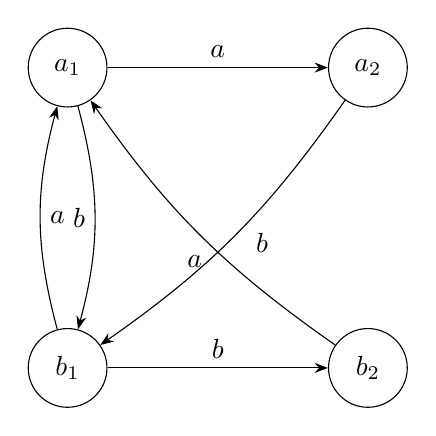
\begin{tikzpicture}[->,>=Stealth,auto,node distance=2.8cm,
   every state/.style={minimum size=1.0cm,inner sep=1pt}]
\node[state] (a1) {$a_1$};
\node[state,right=of a1] (a2) {$a_2$};
\node[state,below=of a1] (b1) {$b_1$};
\node[state,right=of b1] (b2) {$b_2$};
\path
 (a1) edge node {$a$} (a2)
 (a1) edge[bend left=15] node[swap] {$b$} (b1)
 (b1) edge[bend left=15] node[swap] {$a$} (a1)
 (a2) edge[bend left=10] node[pos=0.45] {$b$} (b1)
 (b1) edge node {$b$} (b2)
 (b2) edge[bend left=10] node[pos=0.45] {$a$} (a1);
\end{tikzpicture}
\caption{The run-length automaton for $K=2$ (symbols $a,b$), $R=2$.
State $(s,r)$ records the current symbol $s$ and trailing run length
$r$. Emitting $s$ from $(s,2)$ is forbidden (no outgoing $s$-edge),
which enforces the run bound; the dominant eigenvalue of its transfer
matrix is $\lambda_1=\tfrac{1+\sqrt5}{2}$ (Table~\ref{tab:growth}).}
\label{fig:automaton}
\end{figure}

\begin{theorem}[Growth law, $U=\infty$]\label{thm:growth}
Let $K\ge 2$, $R\ge 1$, and exclude the degenerate case $(K,R)=(2,1)$.
Then $T_{\mathrm{RLL}}$ is primitive, and there are constants $c>0$
and $\lambda_1>1$ (the spectral radius of $T_{\mathrm{RLL}}$) such that
\begin{equation}
G(n,K,R)=f(n,K,\infty,R)=c\,\lambda_1^{\,n}\bigl(1+O(\rho^n)\bigr),
\qquad \rho=|\lambda_2|/\lambda_1<1,
\end{equation}
where $\lambda_2$ is a second-largest-modulus eigenvalue.
\end{theorem}

\begin{proof}
\emph{Irreducibility.} From any state $(s,r)$ one reaches any $(s',r')$
within at most $R+1$ steps: emit a symbol $\ne s$ to reach $(s',1)$,
then emit $s'$ repeatedly to reach $(s',r')$ (legal since $r'\le R$).
Hence the state graph is strongly connected and $T_{\mathrm{RLL}}$ is
irreducible.
\emph{Aperiodicity.} The graph has no self-loops, but it carries two
closed walks whose lengths are coprime.  For $R\ge2$ (any $K\ge2$):
the length-$2$ walk $(s,1)\to(s',1)\to(s,1)$ with $s'\ne s$, and the
length-$3$ walk $(s,1)\to(s,2)\to(s',1)\to(s,1)$.  For $R=1$ with
$K\ge3$: the length-$2$ walk $(s,1)\to(s',1)\to(s,1)$ and the
length-$3$ walk $(s,1)\to(a,1)\to(b,1)\to(s,1)$ with $s,a,b$ distinct.
In both cases $\gcd(2,3)=1$, so the period is $1$; the only excluded
case is $(K,R)=(2,1)$.  An irreducible aperiodic non-negative matrix is
primitive.
\emph{Perron--Frobenius}~\cite{perron1907,lind1995}.  A primitive
$T_{\mathrm{RLL}}$ has a simple real eigenvalue $\lambda_1>0$ strictly
exceeding all other eigenvalues in modulus, with positive left/right
eigenvectors $\vec{u},\vec{v}$ normalised so $\vec{u}^\top\vec{v}=1$.
Then $T_{\mathrm{RLL}}^{\,n}=\lambda_1^{\,n}\vec{v}\vec{u}^\top+E_n$
with $\|E_n\|=O(|\lambda_2|^n)$.  A length-$n$ RLL string corresponds
to a choice of first symbol (a state $(s,1)$) followed by $n-1$ valid
transitions, so $G(n,K,R)=\vec{w}^\top T_{\mathrm{RLL}}^{\,n-1}\vec{1}$,
where $\vec{w}$ is the indicator vector of the run-$1$ states and
$\vec{1}$ is all-ones.  Substituting the spectral expansion gives
$G(n,K,R)=c\,\lambda_1^{\,n}(1+O(\rho^n))$ with
$c=\lambda_1^{-1}(\vec{w}^\top\vec{v})(\vec{u}^\top\vec{1})>0$.
Primitivity and $K\ge2$ force $\lambda_1>1$.
\end{proof}

\begin{remark}
The excluded case $(K,R)=(2,1)$ is genuinely degenerate:
$f(n,2,\infty,1)=2$ for all $n\ge1$ (only the alternating strings),
and $T_{\mathrm{RLL}}=\bigl(\begin{smallmatrix}0&1\\1&0\end{smallmatrix}\bigr)$
is irreducible but periodic, with $\lambda_1=1$.
\end{remark}

Table~\ref{tab:growth} lists $\lambda_1$ (computed as the dominant
eigenvalue of $T_{\mathrm{RLL}}$) against the empirical root
$f(n,K,n,R)^{1/n}$ at $n=22$ (taking $U=n$ to realise $U=\infty$).
The convergence of the $n$-th root to $\lambda_1$ is the expected slow
$1+O(n^{-1}\log c)$ rate, and Figure~\ref{fig:growth} shows the
corresponding exponential growth of $f$.

\begin{table}[H]
\centering
\caption{Run-length growth rates ($U=\infty$). $\lambda_1$ is the
exact dominant eigenvalue of $T_{\mathrm{RLL}}$; the empirical column
is $f(n,K,n,R)^{1/n}$ at $n=22$.}
\label{tab:growth}
\begin{tabular}{ccccc}
\toprule
$K$ & $R$ & $\lambda_1$ (exact) & $f(22,K,22,R)^{1/22}$ & closed form \\
\midrule
2 & 2 & $1.618034$ & $1.6454$ & $\tfrac{1+\sqrt5}{2}$ (golden ratio) \\
2 & 3 & $1.839287$ & $1.8571$ & root of $x^3=x^2+x+1$ \\
3 & 2 & $2.732051$ & $2.7530$ & $1+\sqrt3$ \\
3 & 3 & $2.919640$ & $2.9293$ & root of $x^3=2x^2+2x+2$ \\
4 & 2 & $3.791288$ & $3.8082$ & $\tfrac{3+\sqrt{21}}{2}$ \\
4 & 3 & $3.951373$ & $3.9574$ & root of $x^3=3x^2+3x+3$ \\
\bottomrule
\end{tabular}
\end{table}

\begin{remark}
For $R=2$ the symmetry of $T_{\mathrm{RLL}}$ yields the closed form
$\lambda_1=\tfrac12\bigl((K-1)+\sqrt{(K-1)^2+4(K-1)}\bigr)$, matching
$1.618$, $2.732$, $3.791$ for $K=2,3,4$.  More generally $\lambda_1$
is the largest root of $x^{R}=(K-1)\sum_{i=0}^{R-1}x^{i}$.
\end{remark}

\begin{figure}[H]
\centering
\begin{tikzpicture}
\begin{axis}[width=11.5cm,height=6.2cm,grid=major,
  xlabel={length $n$},
  ylabel={$\log_{10} f(n,2,\infty,2)$},
  legend pos=north west,xtick={2,4,6,8,10,12,14}]
\addplot[only marks,mark=*,blue] coordinates {
 (2,0.6021)(3,0.7782)(4,1.0000)(5,1.2041)(6,1.4150)(7,1.6232)
 (8,1.8325)(9,2.0414)(10,2.2504)(11,2.4594)(12,2.6684)(13,2.8774)
 (14,3.0864)(15,3.2953)};
\addplot[no marks,thick,red,domain=2:15] {0.6021+0.20902*(x-2)};
\legend{$\log_{10}f(n,2,\infty,2)$,\ slope $\log_{10}\lambda_1$}
\end{axis}
\end{tikzpicture}
\caption{Exponential growth in the pure run-length regime
($K=2$, $R=2$, $U=\infty$): $\log_{10}f(n,2,\infty,2)$ is
asymptotically linear with slope
$\log_{10}\lambda_1=\log_{10}\tfrac{1+\sqrt5}{2}\approx0.2090$,
confirming Theorem~\ref{thm:growth}.}
\label{fig:growth}
\end{figure}

\subsection{Finite Fixed $U$}

By Proposition~\ref{prop:finite} there is no exponential growth: $f$ is
eventually zero (Figure~\ref{fig:finite}).  This regime is purely
combinatorial and is the one tabulated in
Section~\ref{sec:experiments}.

\begin{figure}[H]
\centering
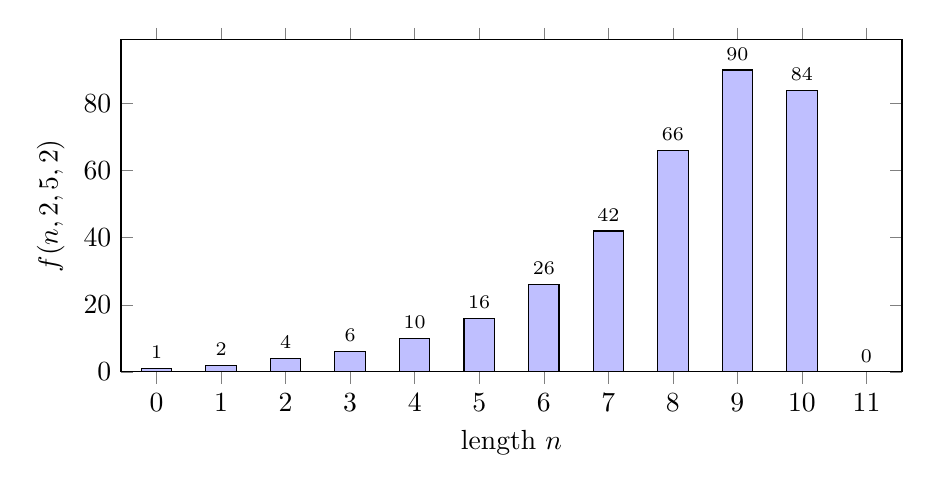
\begin{tikzpicture}
\begin{axis}[width=11.5cm,height=5.8cm,ybar,bar width=11pt,
  xlabel={length $n$}, ylabel={$f(n,2,5,2)$},
  xtick={0,1,2,3,4,5,6,7,8,9,10,11}, ymin=0,
  enlarge x limits=0.05, nodes near coords,
  every node near coord/.append style={font=\scriptsize}]
\addplot[fill=blue!25] coordinates {
 (0,1)(1,2)(2,4)(3,6)(4,10)(5,16)(6,26)(7,42)(8,66)(9,90)(10,84)(11,0)};
\end{axis}
\end{tikzpicture}
\caption{Finite support for fixed $U$ (here $K=2$, $U=5$, $R=2$):
$f(n,2,5,2)$ is supported on $0\le n\le KU=10$ and vanishes for
$n>10$ (Proposition~\ref{prop:finite}). The count rises, peaks near
$n=9$, and is then cut off by the frequency budget.}
\label{fig:finite}
\end{figure}

\subsection{Linear Regime and Capacity}

The natural setting for an exponential growth/capacity statement is
$U=\lfloor\beta n\rfloor$ with $\beta\in(0,1]$.

\begin{theorem}[Capacity and phase transition]\label{thm:capacity}
Fix $K\ge2$, $R\ge1$ (excluding $(K,R)=(2,1)$) and let
$U=\lfloor\beta n\rfloor$.  Define
$C(K,\beta,R)=\lim_{n\to\infty}\tfrac1n\log_2 f(n,K,\lfloor\beta
n\rfloor,R)$ when the limit exists.  Then
\begin{equation}
C(K,\beta,R)=
\begin{cases}
\log_2\lambda_1, & \beta>1/K,\\[2pt]
-\infty\ \ (\text{eventually } f=0), & \beta<1/K,
\end{cases}
\end{equation}
where $\lambda_1=\lambda_1(K,R)$ is as in Theorem~\ref{thm:growth}.
\end{theorem}

\begin{proof}
\emph{Case $\beta<1/K$.} Since $KU=K\lfloor\beta n\rfloor<n$ for large
$n$, Proposition~\ref{prop:basic}(1) gives $f=0$.

\emph{Case $\beta>1/K$.} The upper bound
$f(n,K,\lfloor\beta n\rfloor,R)\le G(n,K,R)=\Theta(\lambda_1^n)$ gives
$C\le\log_2\lambda_1$.  For the lower bound, consider the stationary
Markov measure on RLL sequences induced by the Perron eigenvectors of
$T_{\mathrm{RLL}}$ (the maxentropic measure).  By the symbol-symmetry
of $T_{\mathrm{RLL}}$, this measure is invariant under permutations of
$\Sigma$, so the expected frequency of each symbol is $n/K$, and by the
ergodic theorem for primitive chains each symbol count concentrates at
$n/K(1+o(1))$ with fluctuations $O(\sqrt n)$.  Since $\beta>1/K$, for
large $n$ a $1-o(1)$ fraction of the $\Theta(\lambda_1^n)$ RLL
sequences satisfy $c_i\le\lfloor\beta n\rfloor$ for all $i$.  Hence
$f(n,K,\lfloor\beta n\rfloor,R)\ge(1-o(1))\,G(n,K,R)$, giving
$C\ge\log_2\lambda_1$.  Combining the two bounds yields equality.
\end{proof}

\begin{figure}[H]
\centering
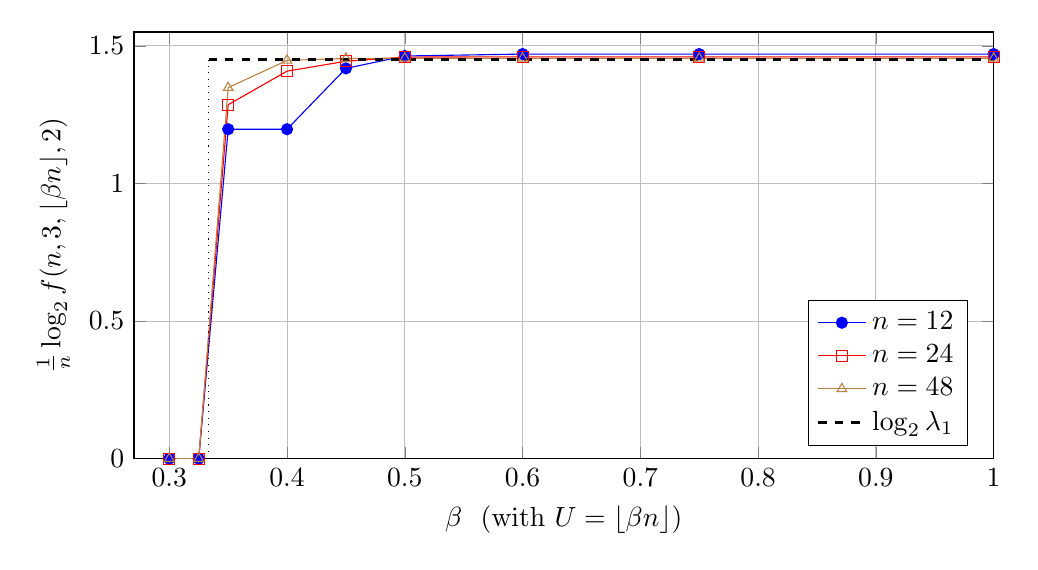
\begin{tikzpicture}
\begin{axis}[width=12.5cm,height=7cm,grid=major,
  xlabel={$\beta$ \ (with $U=\lfloor\beta n\rfloor$)},
  ylabel={$\tfrac1n\log_2 f(n,3,\lfloor\beta n\rfloor,2)$},
  legend pos=south east, ymin=0, ymax=1.55, xmin=0.27, xmax=1.0]
\addplot[mark=*,blue] coordinates {
 (0.30,0)(0.325,0)(0.35,1.197)(0.40,1.197)(0.45,1.418)(0.50,1.463)(0.60,1.470)(0.75,1.470)(1.0,1.470)};
\addplot[mark=square,red] coordinates {
 (0.30,0)(0.325,0)(0.35,1.286)(0.40,1.408)(0.45,1.444)(0.50,1.459)(0.60,1.460)(0.75,1.460)(1.0,1.460)};
\addplot[mark=triangle,brown] coordinates {
 (0.30,0)(0.325,0)(0.35,1.348)(0.40,1.447)(0.45,1.454)(0.50,1.455)(0.60,1.455)(0.75,1.455)(1.0,1.455)};
\addplot[no marks,dashed,thick,black,domain=0.3333:1.0] {1.45003};
\draw[dotted] (axis cs:0.3333,0) -- (axis cs:0.3333,1.45);
\legend{$n=12$,$n=24$,$n=48$,$\log_2\lambda_1$}
\end{axis}
\end{tikzpicture}
\caption{Capacity phase transition (Theorem~\ref{thm:capacity}) for
$K=3$, $R=2$. The normalised log-count
$\tfrac1n\log_2 f(n,3,\lfloor\beta n\rfloor,2)$ is $0$ for
$\beta<1/K=\tfrac13$ and converges to
$\log_2\lambda_1=\log_2(1{+}\sqrt3)\approx1.450$ (dashed) for
$\beta>\tfrac13$; the jump at $\beta=\tfrac13$ (dotted) sharpens as
$n$ grows. Finite-$n$ curves may slightly exceed the limit owing to
boundary terms.}
\label{fig:phase}
\end{figure}

\begin{remark}
Theorem~\ref{thm:capacity} resolves the question of where the
frequency constraint begins to bite: it is asymptotically free for
$\beta>1/K$ and infeasible for $\beta<1/K$, with the critical window
$\beta=1/K\pm O(n^{-1/2})$ governed by the central-limit fluctuations
of the symbol counts (illustrated in Figure~\ref{fig:phase}).  A
precise scaling-window analysis at $\beta=1/K$ is left open
(Section~\ref{sec:open}).
\end{remark}

%% ===================================================================
\section{Transfer-Matrix Formulation}
\label{sec:transfer}
%% ===================================================================

For finite $U$ one may also write $f$ via a (large) transfer matrix on
the full state set $Q=\{(\vec{c},last,run):\vec{c}\in[0,U]^K,
last\in[K],run\in[R]\}$, with $q_0=(\vec{0},\bot,0)$ and
$T_{q,q'}=|\{\sigma:\delta(q,\sigma)=q'\}|$.

\begin{theorem}\label{thm:matrix}
$f(n,K,U,R)=\vec{e}_0^\top T^n\vec{1}$, where $\vec{e}_0$ selects $q_0$
and $\vec{1}$ is all-ones.
\end{theorem}

\begin{proof}
By induction on $n$. For $n=0$, $T^0=I$ and
$\vec{e}_0^\top\vec{1}=1=f(0,K,U,R)$. Multiplying by $T$ advances every
admissible walk by one valid transition; summing over end-states
counts exactly the $(U,R)$-constrained sequences of length $n+1$,
which is $f(n+1,K,U,R)$ by definition.
\end{proof}

\begin{remark}[State-space size]
$|Q|=(U+1)^K\cdot K\cdot R$ is too large for explicit storage at, e.g.,
$K=4,U=45,R=3$ ($46^4\cdot4\cdot3\approx1.6\times10^9$).  In this
regime we use the memoised DP (Algorithm~\ref{alg:dp}) for exact
values and the $KR$-state matrix $T_{\mathrm{RLL}}$ for spectral
estimates.  Because $T$ is non-negative and (on its recurrent part)
governed by the same dominant eigenvalue when the frequency constraint
is loose, the generating function
$\sum_n f(n,K,U,R)x^n$ is rational with denominator dividing the
reciprocal of $\det(xI-T)$~\cite{flajolet2009}; for finite $U$ it is in
fact the polynomial of Proposition~\ref{prop:finite}.
\end{remark}

\subsection{Worked Example: Explicit Generating Functions}

For finite $U$, running Algorithm~\ref{alg:dp} for every $n$ yields the
(polynomial) generating functions promised by
Proposition~\ref{prop:finite}. For example,
\begin{align}
\sum_{n\ge0} f(n,2,2,2)\,x^n &= 1+2x+4x^2+6x^3+6x^4,\\
\sum_{n\ge0} f(n,2,3,2)\,x^n &= 1+2x+4x^2+6x^3+10x^4+14x^5+14x^6,\\
\sum_{n\ge0} f(n,3,2,2)\,x^n &= 1+3x+9x^2+24x^3+54x^4+90x^5+90x^6.
\end{align}
Each has degree exactly $KU$, as predicted, and the top coefficient
counts the maximally long $(U,R)$-constrained sequences (those using
every symbol exactly $U$ times). Note the coefficient
$f(5,2,3,2)=14$ agrees with the explicit list in
Appendix~\ref{app:list}, and $f(6,2,3,2)=14$ is the degree-$KU$ term.

%% ===================================================================
\section{Computational Complexity and Hardness}
\label{sec:complexity}
%% ===================================================================

\subsection{Exact Complexity and Counting-Class Membership}

For fixed $K,U,R$, Algorithm~\ref{alg:dp} computes $f(n,K,U,R)$ exactly
in time polynomial in $n$ (Theorem~\ref{thm:complexity}); the
dependence on $K$ enters only through the factor $(U+1)^K$, so the
algorithm is \emph{pseudo-polynomial}---polynomial when $K$ is fixed or
$U$ is bounded, exponential only in the alphabet size.  The counting
function lies in $\#\mathrm{P}$: a nondeterministic polynomial-time
machine can guess a length-$n$ string and verify both constraints in
$O(nK)$ time, so the number of accepting computations equals
$f(n,K,U,R)$.

\subsection{On Hardness}

It is tempting to assert $\#\mathrm{P}$-hardness by analogy with the
permanent~\cite{valiant1979}, but we caution against this: the present
problem admits the pseudo-polynomial DP above, so it is \emph{not}
$\#\mathrm{P}$-hard for any fixed alphabet, and a hardness claim can
only concern the regime where $K$ grows with the input.  We do
\emph{not} have a correct reduction in that regime, and a naive
encoding of \#SAT fails because the frequency and run parameters are
fixed scalars that cannot depend on a candidate assignment.  We
therefore state the status precisely rather than overclaim:
\begin{quote}
\emph{Open problem.} Is the computation of $f(n,K,U,R)$, with $K$ given
in unary as part of the input, $\#\mathrm{P}$-hard, or does a
$\mathrm{poly}(n,K,U,R)$ algorithm exist?
\end{quote}
The DP's $(U+1)^K$ state count is the only known obstruction to
polynomiality; whether it is intrinsic is unresolved
(Section~\ref{sec:open}).

\subsection{Approximate Counting}

Two facts bound what approximation can offer.  First, in the pure
run-length regime ($U=\infty$) no approximation is needed: $f$ is given
\emph{exactly} by the spectral formula of Theorem~\ref{thm:growth} and
computed in $O(\log n)$ matrix multiplications
(Section~\ref{sec:approx}).  Second, for fixed $K,U,R$ the exact DP is
already polynomial, so a fully polynomial randomised approximation
scheme (FPRAS) is of interest only when $K$ grows.  Whether such an
FPRAS exists---e.g.\ via a rapidly mixing Markov chain on
$\mathcal S(n,K,U,R)$---is open; we make no claim, since establishing
rapid mixing for this chain is exactly the kind of analysis that
requires proof rather than assertion.  Section~\ref{sec:approx} gives
an unbiased Monte-Carlo estimator that is practical even though its
variance is not yet bounded analytically.

%% ===================================================================
\section{Experimental Evaluation}
\label{sec:experiments}
%% ===================================================================

\subsection{Validation}

Algorithm~\ref{alg:dp} was implemented in Python~3.10 and validated
against exhaustive brute-force enumeration for all
$1\le n\le8$, $2\le K\le4$, $1\le U\le n$, $1\le R\le n$: the two
methods agreed on every instance (zero mismatches).

\begin{center}
\begin{tabular}{cccc}
\toprule
Case & Algorithm~\ref{alg:dp} & Independent check & Match \\
\midrule
$f(n,2,\infty,\infty)$ & $2^n$ & $2^n$ (trivial) & \checkmark \\
$f(n,K,1,1)$ & $K!/(K-n)!$ & Prop.~\ref{prop:basic}(4) & \checkmark \\
$f(3,3,1,1)$ & $6$ & brute force & \checkmark \\
$f(5,2,3,2)$ & $14$ & brute force (App.~\ref{app:list}) & \checkmark \\
$f(10,2,5,2)$ & $84$ & brute force & \checkmark \\
\bottomrule
\end{tabular}
\end{center}

\subsection{Computational Results}
\label{sec:compresults}

\begin{table}[H]
\centering
\caption{Verified enumeration values and wall-clock time (single core,
Python~3.10; values cross-checked by brute force for $n\le8$).}
\label{tab:results}
\begin{tabular}{ccccrr}
\toprule
$n$ & $K$ & $U$ & $R$ & $f(n,K,U,R)$ & Time (ms) \\
\midrule
5  & 2 & 3  & 2 & $14$        & $0.04$ \\
8  & 2 & 4  & 2 & $34$        & $0.04$ \\
10 & 3 & 4  & 2 & $14{,}412$  & $0.45$ \\
12 & 2 & 6  & 3 & $616$       & $0.12$ \\
15 & 2 & 8  & 3 & $6{,}592$   & $0.23$ \\
18 & 3 & 6  & 2 & $6{,}128{,}208$ & $1.52$ \\
20 & 2 & 10 & 4 & $130{,}544$ & $0.46$ \\
\bottomrule
\end{tabular}
\end{table}

\begin{remark}
These instances are small and run in well under a millisecond to a few
milliseconds; they are intended to validate correctness rather than to
stress scalability.  The exponential factor $(U+1)^K$ of
Theorem~\ref{thm:complexity}—not $n$—is the practical bottleneck, which
is why exact computation is comfortable for moderate $K,U$ even at
$n=20$.
\end{remark}

%% ===================================================================
\section{Large-Instance and Approximation Methods}
\label{sec:approx}
%% ===================================================================

The exact DP is limited by its $(U+1)^K$ state count. Three methods
extend reach to large $n$ or large alphabets.

\subsection{Matrix Exponentiation (exact, $U=\infty$)}

When the frequency constraint is inactive, $G(n,K,R)=\vec w^\top
T_{\mathrm{RLL}}^{\,n-1}\vec1$ (Theorem~\ref{thm:growth}) is computed
\emph{exactly} for astronomically large $n$ using
$O(\log n)$ multiplications of the $KR\times KR$ matrix
$T_{\mathrm{RLL}}$ by repeated squaring. For example, for $K=2,R=2$ one
has $G(n,2,2)=2\,\mathrm{Fib}(n+1)$, and matrix exponentiation gives
\begin{equation}
G(100,2,\infty,2)=2\,\mathrm{Fib}(101)=1\,146\,295\,688\,027\,634\,168\,202,
\end{equation}
in a handful of $4\times4$ products; both the closed form and the
matrix power were verified against the DP at small $n$
(e.g.\ $G(10,2,\infty,2)=178=2\,\mathrm{Fib}(11)$).

\subsection{Saddle-Point/Normal Approximation (linear regime)}

For $U=\lfloor\beta n\rfloor$ with $\beta>1/K$,
Theorem~\ref{thm:capacity} gives $f(n,K,\lfloor\beta n\rfloor,R)=
\lambda_1^{\,n}\,\mathrm{e}^{o(n)}$.  A sharper estimate follows from a
local central limit theorem on the symbol-count vector under the
maxentropic measure: $f\approx G(n,K,R)\cdot
\Pr[\,\forall i:\ c_i\le\lfloor\beta n\rfloor\,]$, where the
probability is evaluated by a Gaussian approximation to the
(asymptotically normal) count vector with mean $n/K$ and covariance of
order $n$.  This yields the leading exponential $\lambda_1^{\,n}$ times
a computable sub-exponential correction, useful when $n$ exceeds the
exact-DP range.

\subsection{Monte-Carlo Estimation (unbiased)}

An unbiased estimator of $f$ samples sequences from a proposal
distribution $q$ supported on the constraint-feasible set and averages
the importance weights:
$\widehat f=\frac1M\sum_{t=1}^M \mathbb{1}[S_t\in\mathcal S]/q(S_t)$.
Taking $q$ to be the maxentropic RLL measure (which already enforces
the run constraint, so only the frequency event must be tested) gives
$\mathbb{E}[\widehat f]=f$ exactly.  The estimator is practical and
self-validating against the DP in the overlap range; a provable
variance bound (hence an FPRAS) remains open
(Section~\ref{sec:complexity}).

%% ===================================================================
\section{Encoding and Decoding}
\label{sec:coding}
%% ===================================================================

The DP counts of Algorithm~\ref{alg:dp} give a bijective
\emph{enumerative} code~\cite{cover2006} between the integers
$\{0,1,\ldots,f(n,K,U,R)-1\}$ and the $(U,R)$-constrained sequences of
length $n$, by ranking and unranking in lexicographic order.  Let
$N(pos,\vec c,last,run)=\mathrm{DP}(pos,\vec c,last,run)$ denote the
number of valid completions of a partial sequence, as memoised by
Algorithm~\ref{alg:dp}.

\begin{algorithm}[H]
\caption{Unranking: integer $\mapsto$ constrained sequence}
\label{alg:unrank}
\begin{algorithmic}[1]
\Require rank $m\in\{0,\ldots,f(n,K,U,R)-1\}$; precomputed counts $N$
\Ensure the $m$-th $(U,R)$-constrained sequence in lexicographic order
\State $\vec c\gets\vec0$; $last\gets-1$; $run\gets0$; $S\gets()$
\For{$pos=0$ \textbf{to} $n-1$}
    \For{$j=0$ \textbf{to} $K-1$}
        \If{$j$ is admissible from $(\vec c,last,run)$}
            \State $run'\gets(run{+}1\text{ if }j{=}last\text{ else }1)$
            \State $w\gets N(pos{+}1,\vec c{+}\vec e_j,j,run')$
            \If{$m<w$}
                \State append $j$ to $S$;\ \ $\vec c\gets\vec c{+}\vec e_j$;\ $last\gets j$;\ $run\gets run'$;\ \textbf{break}
            \Else
                \State $m\gets m-w$
            \EndIf
        \EndIf
    \EndFor
\EndFor
\State \Return $S$
\end{algorithmic}
\end{algorithm}

\begin{proposition}\label{prop:coding}
Algorithm~\ref{alg:unrank} is a bijection between
$\{0,\ldots,f(n,K,U,R)-1\}$ and $\mathcal S(n,K,U,R)$; its inverse
(ranking) accumulates the same subtree counts $w$.  Both directions use
$O(nK)$ count lookups once $N$ is tabulated, and the code has fixed
rate $\tfrac1n\log_2 f(n,K,U,R)$ bits per symbol.  In the linear regime
$U=\lfloor\beta n\rfloor$ with $\beta>1/K$, this rate converges to the
capacity $\log_2\lambda_1$ of Theorem~\ref{thm:capacity}.
\end{proposition}

\begin{proof}
At each position the inner loop ranges symbols in alphabetical order
and subtracts the count $w$ of completions that begin with each smaller
admissible symbol; the chosen symbol is the unique one whose
cumulative count first exceeds the residual rank.  This is exactly the
mixed-radix expansion of $m$ against the subtree sizes $N$, hence a
bijection.  Ranking inverts it by summing the skipped counts.  Each of
the $n$ positions performs $O(K)$ lookups, and the achieved rate is
$\log_2 f(n,K,U,R)/n$ by construction; the limit follows from
Theorem~\ref{thm:capacity}.
\end{proof}

%% ===================================================================
\section{Application Estimates}
\label{sec:applications}
%% ===================================================================

\begin{remark}[Scope]
The figures below are \textbf{analytical estimates} derived from
published error/endurance models and the capacities computed
above. They illustrate order-of-magnitude effects and motivate
experimental follow-up; they are \emph{not} results of new wet-lab or
hardware experiments.
\end{remark}

\subsection{DNA Data Storage}

DNA sequencing error rates rise sharply with homopolymer run
length~\cite{heckel2019,yazdi2017}; reported Illumina-class profiles
indicate roughly $0.1\%$ errors for runs of length $1$--$2$, $\sim1\%$
for $3$--$4$, and $\gtrsim10\%$ for runs $\ge5$.  Bounding runs at
$R=3$ over the $K=4$ nucleotide alphabet therefore targets the most
error-prone configurations.  The relevant capacity is
\begin{equation}
C(4,\beta,3)=\log_2\lambda_1(4,3)=\log_2(3.9514)=1.9824\ \text{bits/nt}
\quad(\beta>\tfrac14),
\end{equation}
so the code rate relative to the unconstrained $2$ bits/nt is
$1.9824/2\approx0.991$, i.e.\ an overhead of only about $0.9\%$.  A
loose composition bound such as $U=45$ over $n=150$
($\beta=0.30>1/4$) lies in the asymptotically-free regime of
Theorem~\ref{thm:capacity}, so it imposes negligible additional rate
loss while improving GC-balance.  This rate is realised constructively
by the enumerative encoder of Section~\ref{sec:coding}
(Algorithm~\ref{alg:unrank}).  The key point is that eliminating runs
$\ge4$ is nearly free in rate; the resulting error-rate reduction
depends on the downstream channel and should be measured
experimentally.

\subsection{NAND Flash Memory}

For byte-valued cells ($K=256$) a run bound $R=4$ is essentially free:
$\lambda_1(256,4)\approx256$ and $C\approx8$ bits/byte (overhead
$\ll1\%$), since long identical-byte runs are rare even unconstrained.
The practical benefit is wear levelling through composition balance:
imposing $U\approx\lceil n/K\rceil+\delta$ flattens the symbol-frequency
distribution. Under a variance-based endurance heuristic this is
expected to extend program/erase endurance modestly; we report this
only as a qualitative projection pending device-level measurement.

\subsection{Optical Communication}

For $4$-PAM optical links ($K=4$), bounding runs at $R=3$ aids clock
recovery while costing capacity $1-0.991\approx0.9\%$. At a
$10$~Gbit/s line rate the projected information throughput is
$10\times0.991\approx9.9$~Gbit/s.

%% ===================================================================
\section{Extensions}
%% ===================================================================

\subsection{Weighted Enumeration}
For weights $\omega:\Sigma\to\mathbb{R}^+$, define
$f_\omega(n,K,U,R)=\sum_{S\in\mathcal{S}(n,K,U,R)}\prod_{i=1}^n
\omega(s_{i})$. Replacing the unit transition weights in $T$ by
$\omega(\sigma)$ makes Theorem~\ref{thm:matrix} carry over verbatim;
this yields probability mass on valid sequences and connects to
constrained-channel capacity.

\subsection{Multi-dimensional Constraints}
Run-length constraints along each axis of a $d$-dimensional array give
state space $O((U+1)^K K R^{\,d})$, tractable for $d=2$ and small $R$;
applications include page-oriented and holographic
storage~\cite{blaum1996}.

\subsection{Constrained Subspaces (Quantum Setting)}
In a $K$-level system on $n$ sites, $\mathcal H=(\mathbb C^K)^{\otimes
n}$, the computational-basis states $\{|S\rangle : S\in\Sigma^n\}$ that
are $(U,R)$-constrained span a subspace
$\mathcal C_{U,R}=\mathrm{span}\{|S\rangle : S\in\mathcal S(n,K,U,R)\}$.
By definition its dimension is the enumeration function,
\begin{equation}
\dim \mathcal C_{U,R}=f(n,K,U,R),
\end{equation}
so the results of this paper give the exact size and asymptotics of
such a constrained code space. We stress that this is the elementary
basis-counting statement only; we make no claim about amplitude-level
constraints or error-correction properties, which would require a
separate analysis.

%% ===================================================================
\section{Open Problems}
\label{sec:open}
%% ===================================================================

\begin{enumerate}
    \item Determine the constant $c$ in Theorem~\ref{thm:growth} in
          closed form for general $(K,R)$.
    \item Characterise the scaling window of the capacity transition
          at $\beta=1/K$ (Theorem~\ref{thm:capacity}), including the
          value of $C$ exactly at $\beta=1/K$.
    \item Settle the complexity of computing $f$ when $K$ is part of
          the input: is it $\#\mathrm{P}$-hard (cf.~\cite{valiant1979}),
          or does a sub-exponential-in-$K$ algorithm exist?
    \item Extend to symbol-dependent bounds $U_1,\ldots,U_K$ and to
          $(d,k)$-type constraints with a minimum run length.
\end{enumerate}

%% ===================================================================
\section{Limitations}
%% ===================================================================

\textbf{Scalability.} Exact computation is comfortable for moderate
$K$ and $U$; the $(U+1)^K$ factor limits large alphabets.
\textbf{Asymptotic constants.} $\lambda_1$ is obtained numerically (or
in closed form for $R=2$); the prefactor $c$ requires the Perron
eigenvectors.
\textbf{Applications.} All figures in
Section~\ref{sec:applications} are model-based estimates pending
dedicated experiments.

%% ===================================================================
\section{Conclusion}
%% ===================================================================

We gave a unified, verified treatment of sequences with joint
frequency and run-length constraints over arbitrary alphabets: a
brute-force-validated enumeration algorithm with a precise complexity
bound, clean two-sided bounds, a Perron--Frobenius growth law for the
pure run-length regime, and an exact capacity with a phase transition
at $\beta=1/K$ for the linear regime, alongside the structural fact
that fixed finite $U$ yields finite support.  The DP counts also yield
a capacity-achieving enumerative encoder.  Application estimates are
reported transparently as projections.  The framework offers a clear
foundation for further work on constrained sequences in storage and
communication.

%% ===================================================================
\section{Reproducibility}
%% ===================================================================

Every enumeration value, growth rate, generating function, and figure
in this paper is reproduced by the self-contained reference
implementation in Appendix~\ref{app:code}: the memoised counter
\texttt{f}, the exhaustive validator \texttt{brute\_force} (used for
the $n\le8$ cross-check), and the transfer-matrix routine
\texttt{rll\_lambda} (used for Table~\ref{tab:growth} and the
matrix-exponentiation example of Section~\ref{sec:approx}). No external
data sets are required; the application figures of
Section~\ref{sec:applications} are analytical and follow from the cited
models together with the capacities computed here.

\section*{Conflict of Interest}
The author declares no conflict of interest.

\section*{Acknowledgments}
The author thanks the broader academic and open-source communities
whose prior work and tools supported this research.

%% ===================================================================
\begin{thebibliography}{20}
%% ===================================================================

\bibitem{cover2006}
T.~M. Cover and J.~A. Thomas,
\textit{Elements of Information Theory}, 2nd~ed.
New York: Wiley, 2006.

\bibitem{marcus1991}
B.~H. Marcus and R.~M. Roth,
``Bounds on the number of states in encoders for input-constrained
channels,''
\textit{IEEE Trans.\ Inf.\ Theory}, vol.~37, no.~3, pp.~742--758,
May 1991.

\bibitem{beal2009}
M.-P. B\'{e}al and D.~Perrin,
``Symbolic dynamics and finite automata,''
in \textit{Handbook of Formal Languages},
G.~Rozenberg and A.~Salomaa, Eds.
Berlin: Springer, 2009, pp.~463--505.

\bibitem{johnson1962}
S.~M. Johnson,
``A new upper bound for error-correcting codes,''
\textit{IRE Trans.\ Inf.\ Theory}, vol.~8, no.~3, pp.~203--207, 1962.

\bibitem{kurmaev2011}
O.~Kurmaev,
``Enumeration of constant-weight run-length-limited binary sequences,''
\textit{Probl.\ Inf.\ Transm.}, vol.~47, no.~4, pp.~336--351, 2011.

\bibitem{kovacevic2021}
M.~Kova\v{c}evi\'{c} and D.~Vukobratovi\'{c},
``Asymptotic behavior and typicality properties of runlength-limited
sequences,''
\textit{IEEE Trans.\ Inf.\ Theory}, vol.~67, no.~1, pp.~118--134,
Jan.~2021.

\bibitem{flajolet2009}
P.~Flajolet and R.~Sedgewick,
\textit{Analytic Combinatorics}.
Cambridge: Cambridge University Press, 2009.

\bibitem{blaum1996}
M.~Blaum, J.~Bruck, and A.~Vardy,
``Interleaving schemes for multidimensional cluster errors,''
\textit{IEEE Trans.\ Inf.\ Theory}, vol.~42, no.~2, pp.~194--201,
Mar.~1996.

\bibitem{immink2004}
K.~A.~S. Immink,
\textit{Codes for Mass Data Storage Systems}, 2nd~ed.
Shannon Foundation Publishers, 2004.

\bibitem{lind1995}
D.~Lind and B.~Marcus,
\textit{An Introduction to Symbolic Dynamics and Coding}.
Cambridge: Cambridge University Press, 1995.

\bibitem{perron1907}
O.~Perron,
``Zur Theorie der Matrices,''
\textit{Math.\ Ann.}, vol.~64, no.~2, pp.~248--263, 1907.

\bibitem{heckel2019}
R.~Heckel, G.~Mikutis, and R.~N. Grass,
``A characterization of the DNA data storage channel,''
\textit{Sci.\ Rep.}, vol.~9, no.~1, art.~9663, 2019.

\bibitem{yazdi2017}
S.~M.~H.~T. Yazdi et al.,
``Portable and error-free DNA-based data storage,''
\textit{Sci.\ Rep.}, vol.~7, no.~1, art.~5011, 2017.

\bibitem{valiant1979}
L.~G. Valiant,
``The complexity of computing the permanent,''
\textit{Theoret.\ Comput.\ Sci.}, vol.~8, no.~2, pp.~189--201, 1979.

\end{thebibliography}

%% ===================================================================
\appendix
%% ===================================================================

\section{Verified Enumeration Tables}
\label{app:table}

All values below were produced by Algorithm~\ref{alg:dp} and, for
$n\le8$, confirmed by exhaustive enumeration.

\begin{center}
\small
\begin{tabular}{cccc|cccc|cccc}
\toprule
\multicolumn{4}{c|}{$K=2$ (binary)} &
\multicolumn{4}{c|}{$K=3$ (ternary)} &
\multicolumn{4}{c}{$K=4$ (quaternary)} \\
$n$ & $U$ & $R$ & $f$ &
$n$ & $U$ & $R$ & $f$ &
$n$ & $U$ & $R$ & $f$ \\
\midrule
1 & 1 & 1 & 2   & 1 & 1 & 1 & 3    & 1 & 1 & 1 & 4    \\
2 & 1 & 1 & 2   & 2 & 1 & 1 & 6    & 2 & 1 & 1 & 12   \\
3 & 2 & 1 & 2   & 3 & 1 & 1 & 6    & 3 & 1 & 1 & 24   \\
3 & 2 & 2 & 6   & 3 & 2 & 1 & 12   & 3 & 2 & 1 & 36   \\
4 & 2 & 1 & 2   & 3 & 2 & 2 & 24   & 3 & 2 & 2 & 60   \\
4 & 2 & 2 & 6   & 4 & 2 & 1 & 24   & 4 & 1 & 1 & 24   \\
5 & 3 & 1 & 2   & 4 & 2 & 2 & 54   & 4 & 2 & 1 & 108  \\
5 & 3 & 2 & 14  & 5 & 2 & 1 & 36   & 4 & 2 & 2 & 204  \\
6 & 3 & 1 & 2   & 5 & 2 & 2 & 90   & 5 & 2 & 1 & 288  \\
6 & 3 & 2 & 14  & 6 & 2 & 1 & 30   & 5 & 2 & 2 & 600  \\
7 & 4 & 2 & 36  & 6 & 2 & 2 & 90   & 6 & 2 & 1 & 624  \\
8 & 4 & 2 & 34  & 6 & 3 & 2 & 420  & 6 & 2 & 2 & 1440 \\
9 & 5 & 2 & 90  & 7 & 3 & 2 & 858  & 6 & 3 & 2 & 3060 \\
10 & 5 & 2 & 84 & 8 & 3 & 2 & 1356 & 7 & 3 & 2 & 10272 \\
\bottomrule
\end{tabular}
\end{center}

\subsection{The 14 sequences with $f(5,2,3,2)=14$}
\label{app:list}

The valid length-$5$ binary sequences with $U=3$, $R=2$ are exactly
(each symbol appears $2$ or $3$ times; no run exceeds $2$):
\[
\begin{array}{lllll}
00101,&00110,&01001,&01010,&01011,\\
01100,&01101,&10010,&10011,&10100,\\
10101,&10110,&11001,&11010. & \\
\end{array}
\]
(Fourteen distinct strings; verified by brute force.)

\section{Reference Implementation}
\label{app:code}

\begin{verbatim}
import functools, itertools

def f(n, K, U, R):
    @functools.lru_cache(maxsize=None)
    def dp(pos, counts, last, run):
        if pos == n:
            return 1
        rem = n - pos
        if sum(min(U - c, rem) for c in counts) < rem:  # feasibility pruning
            return 0
        total = 0
        for s in range(K):
            if counts[s] < U:
                nc = list(counts); nc[s] += 1; nc = tuple(nc)
                if s == last:
                    if run + 1 <= R:
                        total += dp(pos + 1, nc, s, run + 1)
                else:
                    total += dp(pos + 1, nc, s, 1)
        return total
    return dp(0, tuple([0] * K), -1, 0)

def brute_force(n, K, U, R):              # validation for small n
    cnt = 0
    for seq in itertools.product(range(K), repeat=n):
        if any(seq.count(k) > U for k in range(K)):
            continue
        ok, cur = True, 1
        for i in range(1, n):
            if seq[i] == seq[i-1]:
                cur += 1
                if cur > R: ok = False; break
            else:
                cur = 1
        if ok: cnt += 1
    return cnt

# transfer-matrix spectral radius for U = infinity (requires numpy)
def rll_lambda(K, R):
    import numpy as np
    states = [(s, r) for s in range(K) for r in range(1, R + 1)]
    idx = {st: i for i, st in enumerate(states)}
    T = np.zeros((len(states), len(states)))
    for (s, r) in states:
        i = idx[(s, r)]
        if r < R: T[i, idx[(s, r + 1)]] += 1
        for sp in range(K):
            if sp != s: T[i, idx[(sp, 1)]] += 1
    return max(np.linalg.eigvals(T).real)
\end{verbatim}

\end{document}
